\chapter{The Southern Receiver and Component Designs}

\section{Motivation}

  \subsection{Block Diagram}

\begin{figure}[ht]
 \centering
 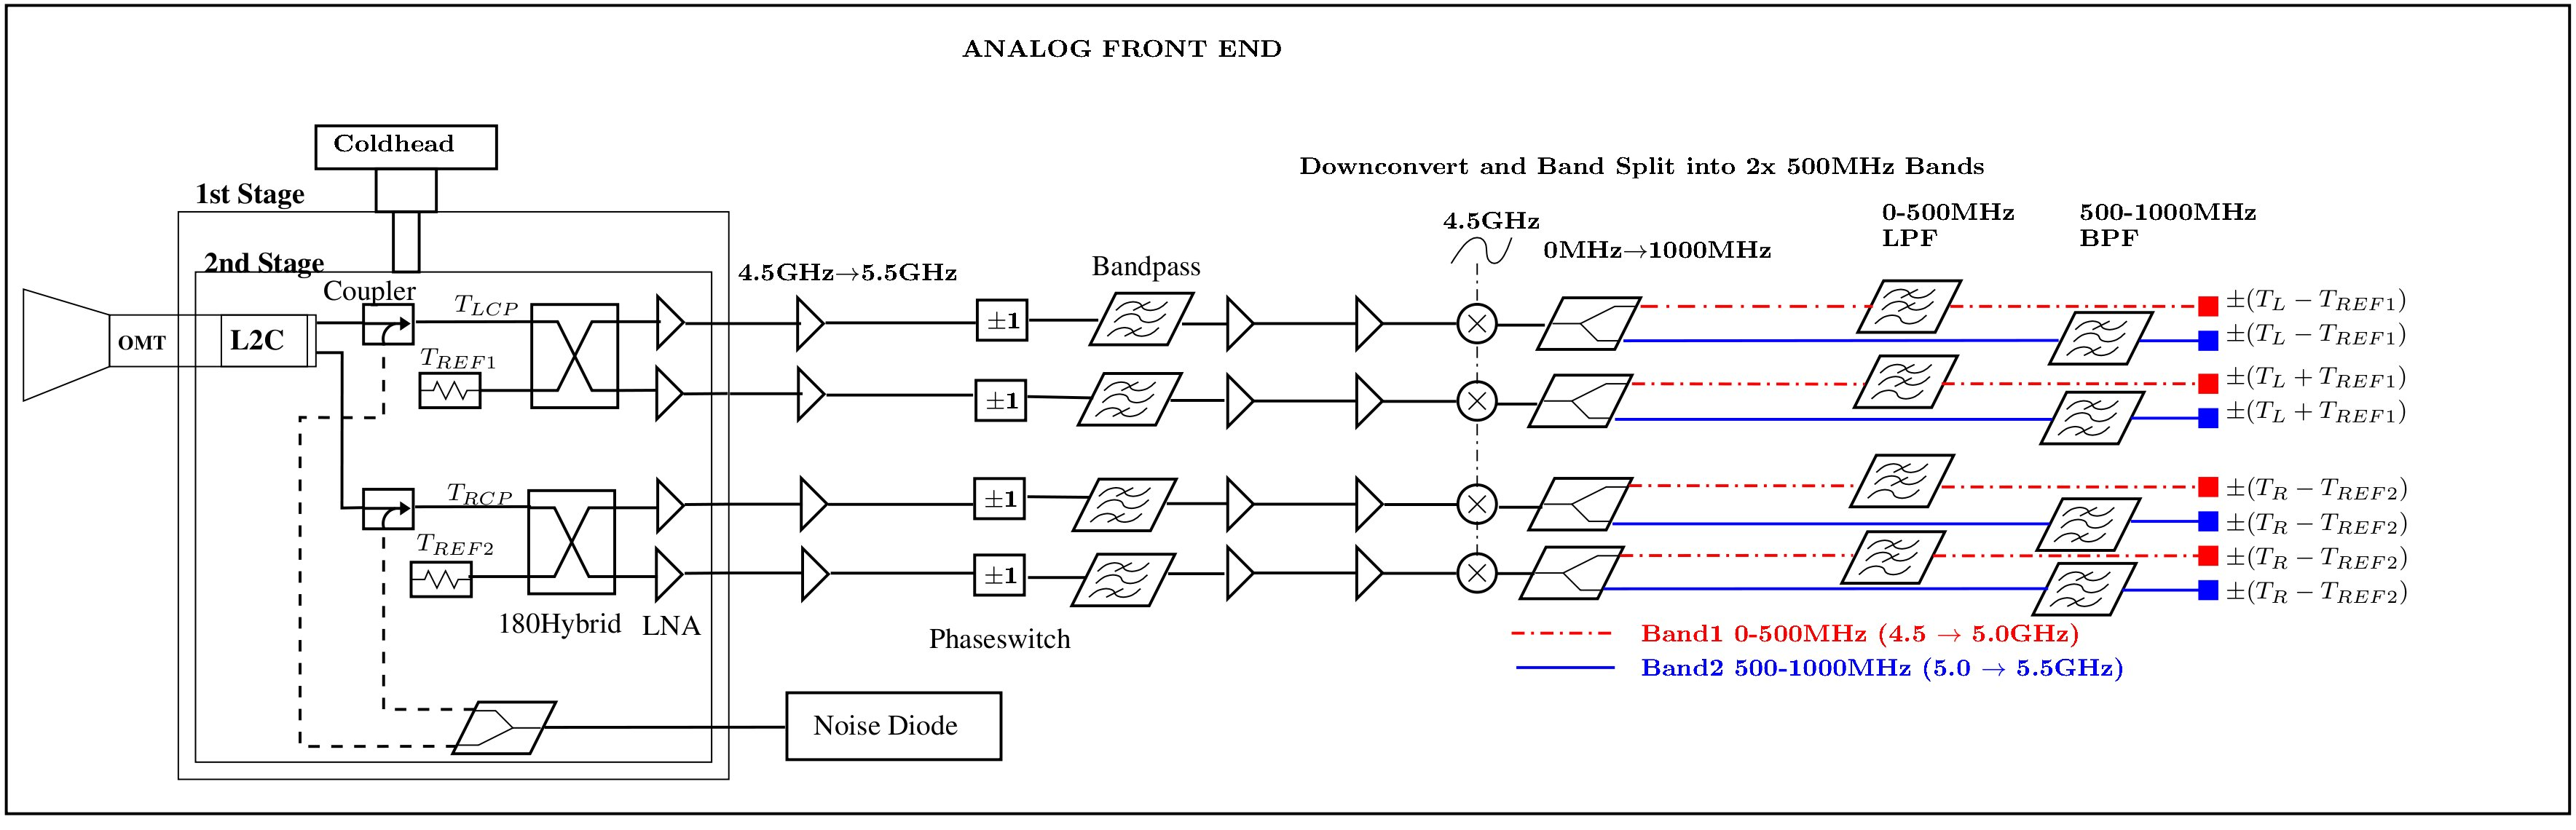
\includegraphics[width=\textwidth,height=0.4\textheight]{images/receiver_schematics/rfNew.jpg} % analog.png: 1920x1200 pixel, 72dpi, 67.73x42.33 cm, bb=
 \caption{Diagram of the analog front end of the digital receiver. There are significantly fewer analog components than the Northern Hemisphere polarimeter (see \appen{sec:pseudoCorrelation}, \fign{fig:analog_receiver}). The diagram shows the down-conversion of the 1~GHz band (into two 500~MHz bands) followed by the ADC capture. The digital processing is shown on \fign{fig:digital_receiver_mine}  }
 \label{fig:digital_receiver}
\end{figure}

\begin{figure}[ht]
 \centering
 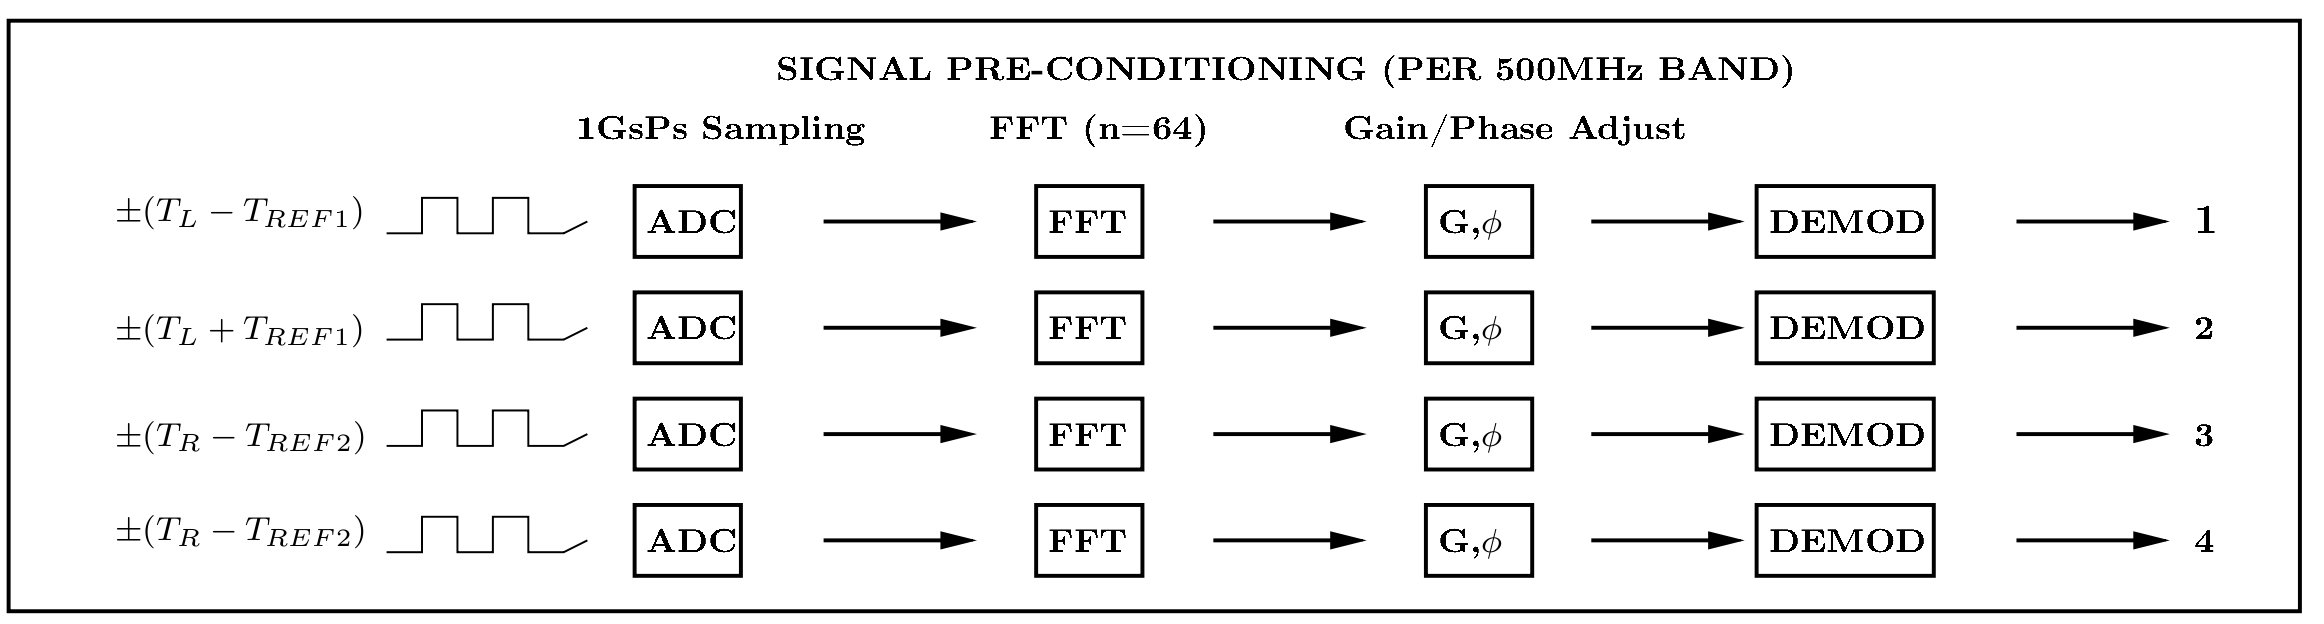
\includegraphics[width=\textwidth]{images/receiver_schematics/precon.jpg}\\
 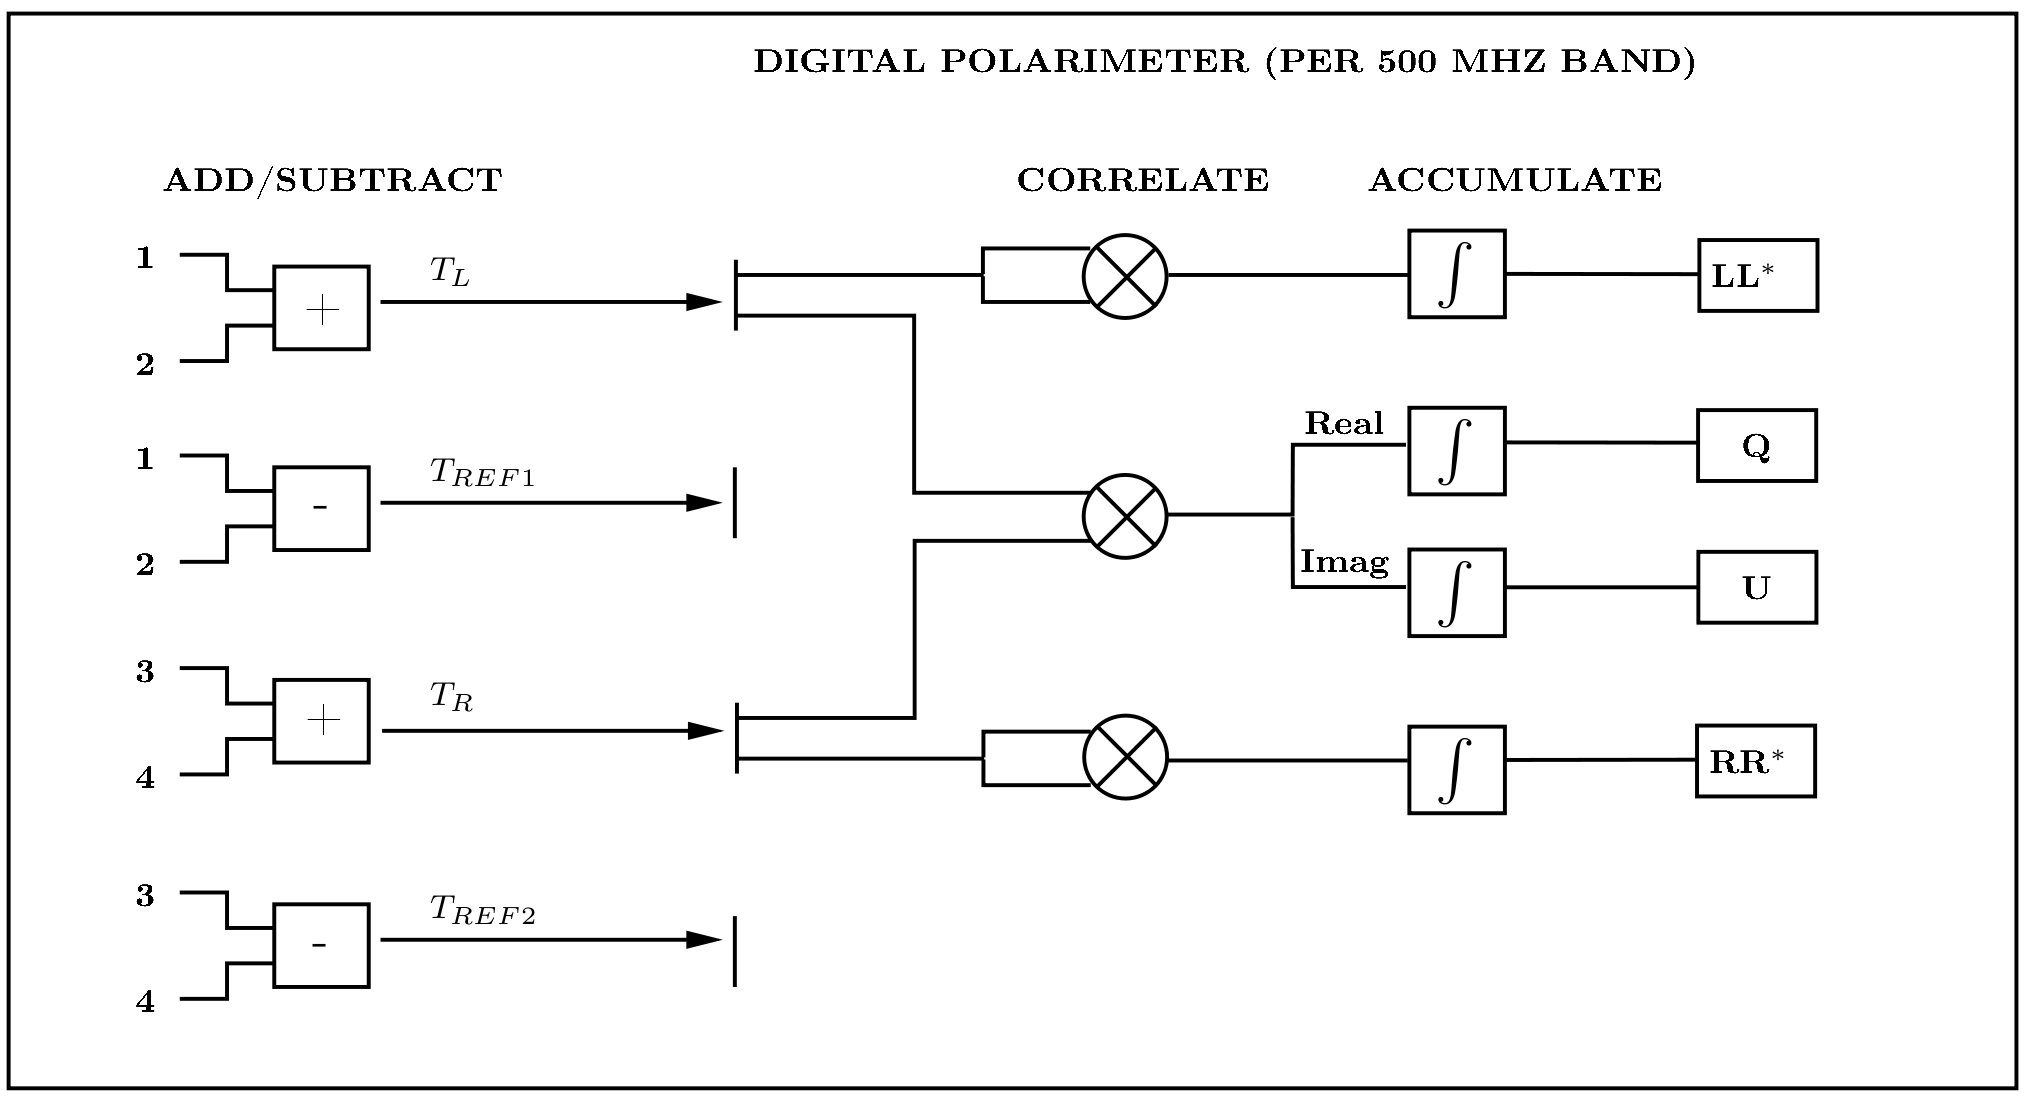
\includegraphics[width=\textwidth]{images/receiver_schematics/roach.jpg}
 % analog.png: 1920x1200 pixel, 72dpi, 67.73x42.33 cm, bb=
 \caption{Diagram of the digital polarimeter. The diagram shows one of the 500~MHz bands. The signals are sampled, fast-Fourier transformed, gain and phase adjusted, demodulated, added, correlated and then accumulated to produce the values required for the Stokes parameters. See \appen{sec:stokes}, Equations~\ref{eq:stokes_circ_I}$\rightarrow$\ref{eq:stokes_circ_V} for clarification on the correlations used to produce the Stokes parameters}
 \label{fig:digital_receiver_mine}
\end{figure}
\clearpage


  \subsection{Designs Choices}


\subsection{Passive Component Insertion Loss}

The system temperature of a radio receiver is given by the \eqn{eq:Friis_Equation}: the Friis Equation.

\begin{equation}
 T_{sys} = T_{sky}+T_{spillover}+T_{optics} + \frac{T_{horn}}{G_{optics}} + \frac{T_{passives}}{G_{optics}G_{horn}}+\frac{T_{LNA}}{G_{optics}G_{horn}G_{passives}}
\label{eq:Friis_Equation}
\end{equation}

The continuous-comparison scheme used in the C-BASS receiver is complicated. The receiver requires significant pre-LNA passive components all of which are lossy. 

From \eqn{eq:Friis_Equation} we see that any pre-LNA loss needs to be avoided. It hurts the system, not just in terms of the individual component resistive noise contribution $(1-L)T_{phys}$, but also in terms of the effect these losses have on subsequent components, in particular the LNA noise contribution, where a 3~dB passive loss will increase the effective noise contribution of the LNA by a factor of 2. 

RF loss takes one of three forms: resistive losses, mismatch losses, dielectric losses. 

Resistive losses hurt the system temperature both by introducing additional noise (proportional to the temperature of the resistor) as well as reducing the signal noise. In a cryogenic radio receiver, losses before the cryostat (warm losses) occur at ~300~K while losses inside the cryostat (cold losses) are at the cryogenic operating temperature (for C-BASS South this is 10~K). We can easily see that the 'warm losses' are best avoided. 

Mismatch losses occur where there is a slight discontinuity in the impedance of the RF path. Classic examples are RF connectors and RF launches onto substrate. Impedance mismatches, cause reflection of the signal, reducing the signal power. These losses do not result in additional noise themselves, but increase the effective noise figure of the amplifier later in the chain.

Dielectric losses occur due to dissipation of electromagnetic energy in the dielectric (effectively heating the dielectric). The losses are proportional to the frequency of the RF.



In the C-BASS architecture, passive loss is difficult to avoid. Consider for a moment the coaxial interconnects between components. One could be forgiven for assuming that the majority of the cable loss resistive, and thus that cooling a coaxial cable assembly (and thus reducing the resistances) will reduce the total cable assembly insertion loss. However this completely ignores the dielectric loss of a coaxial cable and the mismatch loss of the mated connectors. These are not neglible, and need to be understood.

\subsubsection{Coaxial Cable Insertion Loss Model}

\citeasnoun{Pozar2005} models the various we expect in a typical coaxial tranmission line. Here $D$ is the diameter of the outer conductor, and $d$ is the diameter of the inner conductor.

\begin{equation}
 Resistance/length=\left ( \frac{f\mu_{0}}{\pi} \right ) ^{\frac{1}{2}}  \left ( \frac{(\mu_{R1}\rho_{1})^{\frac{1}{2}}}{D} + \frac{(\mu_{R2}\rho_{2})^{\frac{1}{2}}}{d}\right ) 
\label{eq:resistance_length}
\end{equation}

\begin{equation}
 Z_{0}=\frac{138}{\sqrt{\epsilon_{R}}}log \left (\frac{D}{d} \right )
\label{eq:impedance}
\end{equation}

Loss in a coaxial assembly is given by $Loss=Resistance/2Z_{0}$, so combining \eqn{eq:resistance_length} and \eqn{eq:impedance} we arrive at
\begin{eqnarray}
 Loss/length&=&\frac{1}{138 \times 2}\left ( \frac{\epsilon_{R}f\mu_{0}}{\pi} \right ) ^{\frac{1}{2}}  \left ( \frac{(\mu_{R1}\rho_{1})^{\frac{1}{2}}}{D} + \frac{(\mu_{R2}\rho_{2})^{\frac{1}{2}}}{d}\right ) \frac{1}{log\left ( \frac{D}{d} \right )} Np/m\\
\end{eqnarray}

Insertion loss due to dielectric loss of a TEM wave propagating through a coaxial cable as

\begin{equation}
 \alpha_{d}=\frac{\pi \epsilon_{r} tan \delta}{\lambda} Np/m
\label{eq:dielectric_attenuation}
\end{equation}

Another, often omitted loss of a cable assembly, is the connector loss. A typical mated SMA connector has $0.03\sqrt{f_{GHZ}}$~dB ossMeasuring the passive componetns in the cryostat requires careful thought. The ~24hour turnaround between measurements is time intensive and careful consideration needs to be taken to optimise measurments.

The test cable assembly requires initial characterisation. 


\clearpage

\section{Digital Hardware}
\subsection{Roach}

\subsection{iADC}
The iADC is a multi-purpose CASPER analog-to-digital convertor based around the Atmel/e2V AT84AD001B IC. In non-interleaved mode the ADC is capable of sampling 4 signals as 1GsPs i.e a 500~MHz bandwidth. 

\subsubsection{Power Levels}
Tests were carried out to monitor the linearity of the Casper iADC 4-Chann

\subsubsection{Linearity}
\subsubsection{Van Fleck Corrections}

\section{Low Frequency Filters}
AS has been explained, the C-BASS is designed for the 4.5$\rightarrow$5.5~GHz band. This band is defined using edge-coupled filters early in the RF chain. After suitable RF amplification, the signal is downcoverted using a 4.5~GHz LO, mapping 4.5GHz->DC and 5.5GHz to 1~GHz.
In the digital C-BASS we chose to split this 1~GHz band. One iADC/ROACH would sample the first Nyquist Zone (DC-500MHz) and another would sample the second Nyquist Zone (500-1000MHz). We chose to rely on the earlier edge-coupled filters to define the DC and 1GHz roll-off, and required a suitable 500~MHz low pass filter and 500~MHz high pass filter. 

The requirements were small form factor, 20dB roll off in the first 20MHz of band overlap and manufacturability.


\subsection{Filter Design}
\label{sec:lowfreqFilters}

For the design shown in \fign{fig:digital_receiver}, two low frequency filters are required: a 500~MHz lowpass filter and a 500$\rightarrow$1000~MHz bandpass filter.

The difficulty of designing filters in the 1GHz frequency range is that it straddles two design regions \cite{matthaei1980} . Generally higher frequency filters are designed using strip line which scale in size with wavelength making them unsuitable for use at low frequencies. Low frequency designs have tended to use lumped-element capacitors and inductors, but these are notoriously difficult to use at higher frequencies where parasitic effects become important.

The design we have employed uses a lumped-element based approach from  with ongoing development and simulations in the \textit{Microwave Office} software suite. Careful use of standardised, well understood, high quality components has allowed us to build filters at unusually high frequencies usually with rapid turnaround times. This makes use of published component values from Murata \cite{murataAWR}

Results so far are very promising. The 0$\rightarrow$500~MHz Low pass filter is complete (see Figure~\ref{fig:LowFrequency0_500MHz}) and we are rapidly converging on a suitable band-pass filter for the 500$\rightarrow$1000MHz band Figure~\ref{fig:LowFrequency500_1000MHza}. Our understanding of the behaviour of the Murata components at high frequencies has improved significantly since this version of the bandpass filter.



\begin{figure}
 \centering
\subfloat[][Lowpass filter design schematic]{
 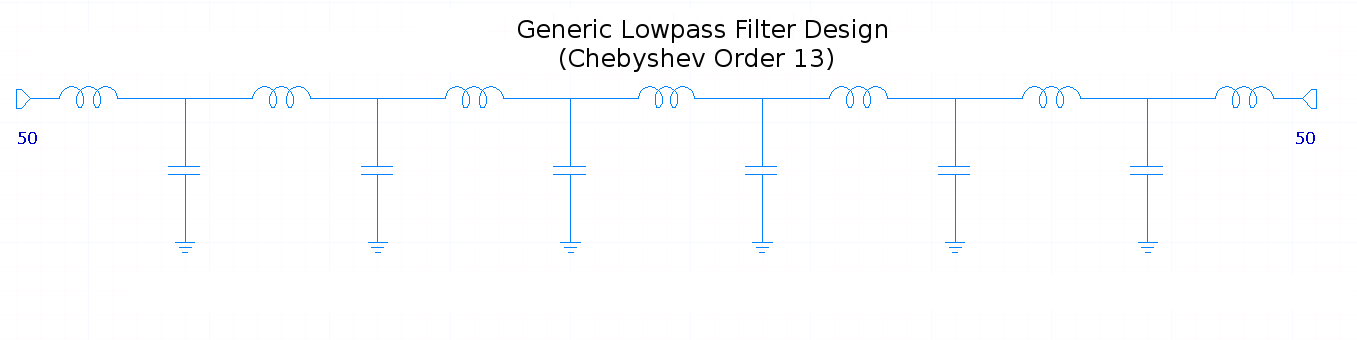
\includegraphics[width=\textwidth]{./images/LowFrequencyFilters/lowpass.png}
}\\
\subfloat[][Bandpass filter design schematic]{
 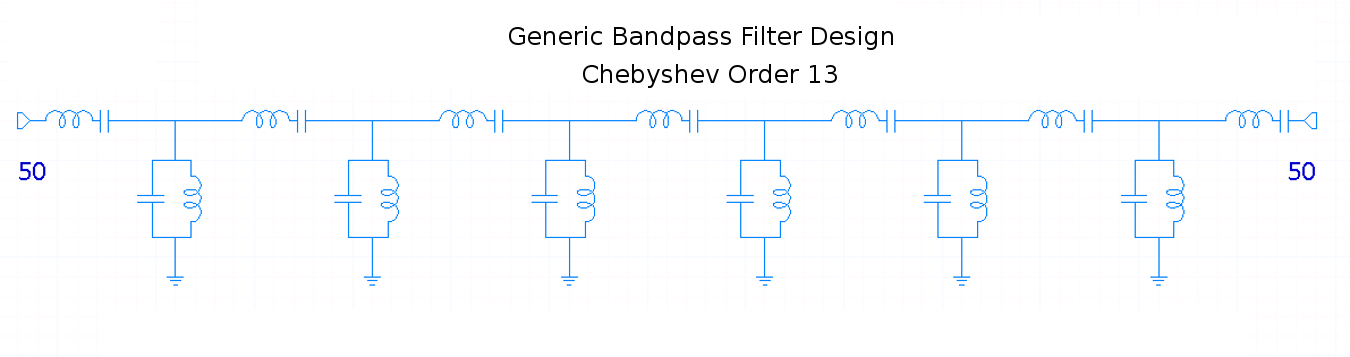
\includegraphics[width=\textwidth]{./images/LowFrequencyFilters/bandpass.png}
}


 % lowpass.png: 1357x340 pixel, 72dpi, 47.87x11.99 cm, bb=0 0 1357 340
 \caption{Low frequency lumped element filter designs and manufacture}
 \label{fig:filterDesigns}
\end{figure}


\begin{figure}
 \centering
\subfloat[][]{
 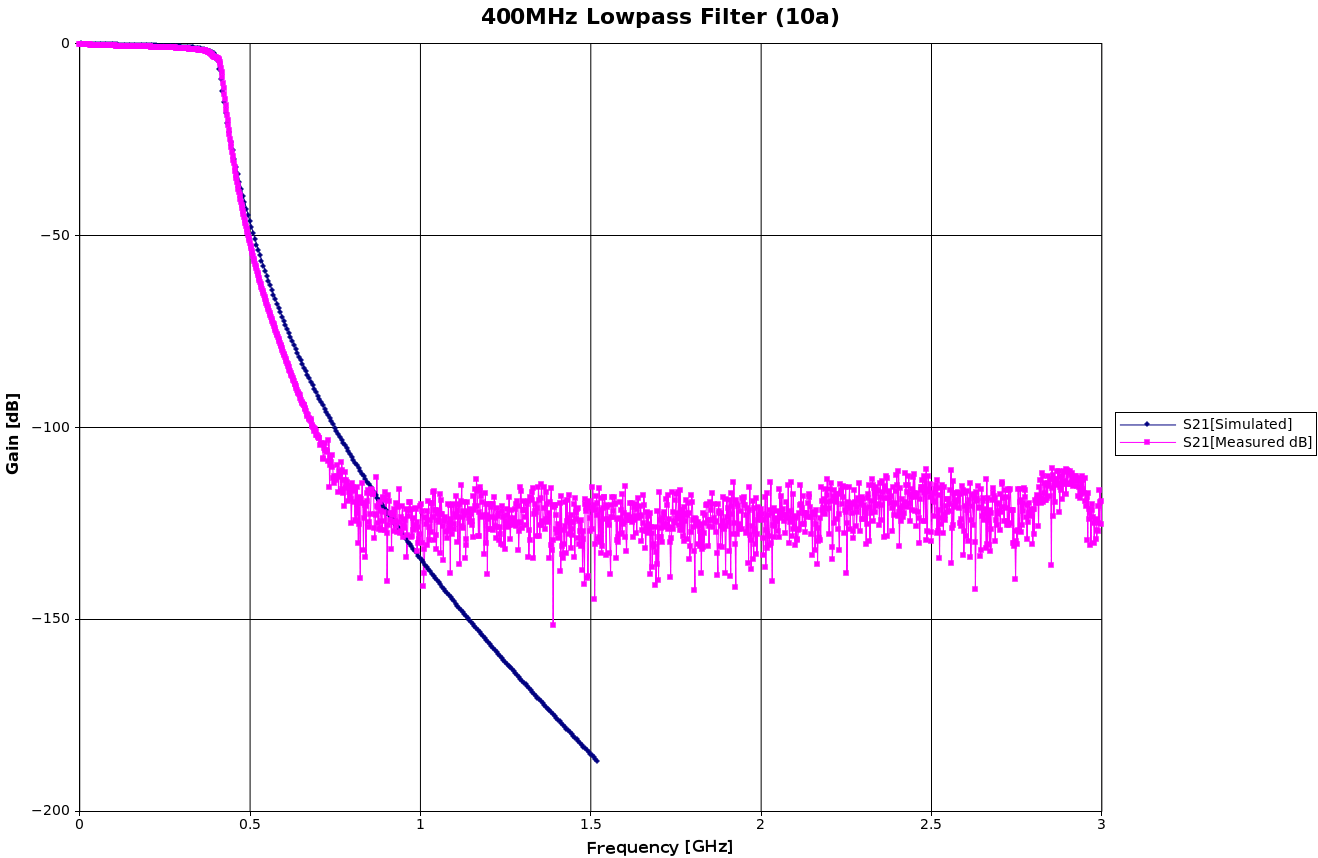
\includegraphics[height=0.4\textheight]{./images/LowFrequencyFilters/lpf10asimvsmeasured1.png}
}\\
\subfloat[][]{
 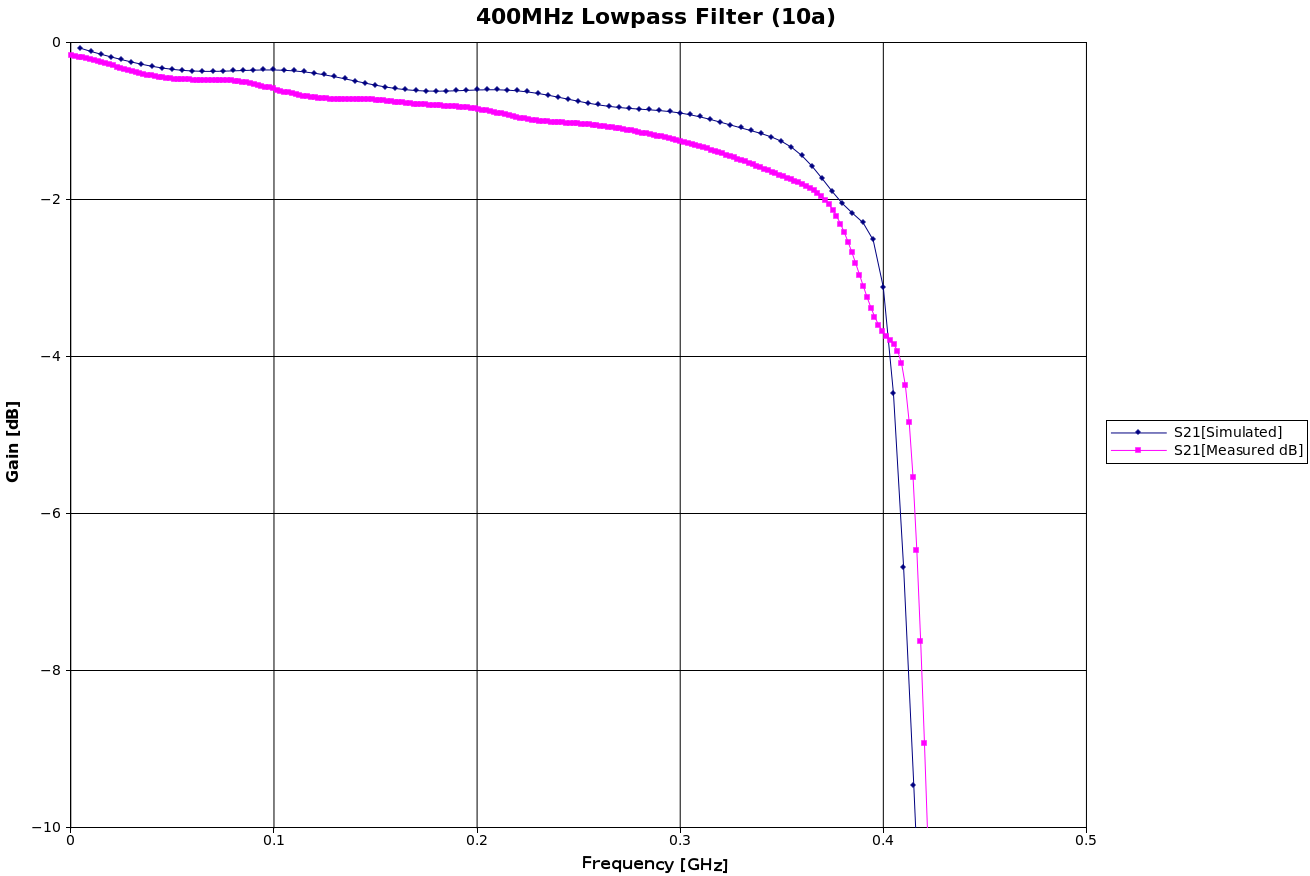
\includegraphics[height=0.4\textheight]{./images/LowFrequencyFilters/lpf10asimvsmeasured2.png}
}
 % lpf10asimvsmeasured1.png: 1571x1046 pixel, 72dpi, 55.41x36.90 cm, bb=0 0 1571 1046
 \caption{Simulated filter performance against measured performance. }
 \label{fig:simvsmeasuredlpf10a}
\end{figure}


We focused on using a design/manufacture technique that would allow rapid prototyping of these filters, and allow quick turnaround times for custom filters that might be required in the future. The techniques we have developed allow a custom filter built in a day, with the major bottleneck still being availability of components. This allows significantly more flexible designs to be produced than was the case previously. In addition, the technique opens up the possibility of building compact filters directly onto printed circuit boards using pick and place for mass production. This has potential for use in large scale radio astronomy deployments such as the Square Kilometer Array. 

% \begin{figure}
%  \centering
%  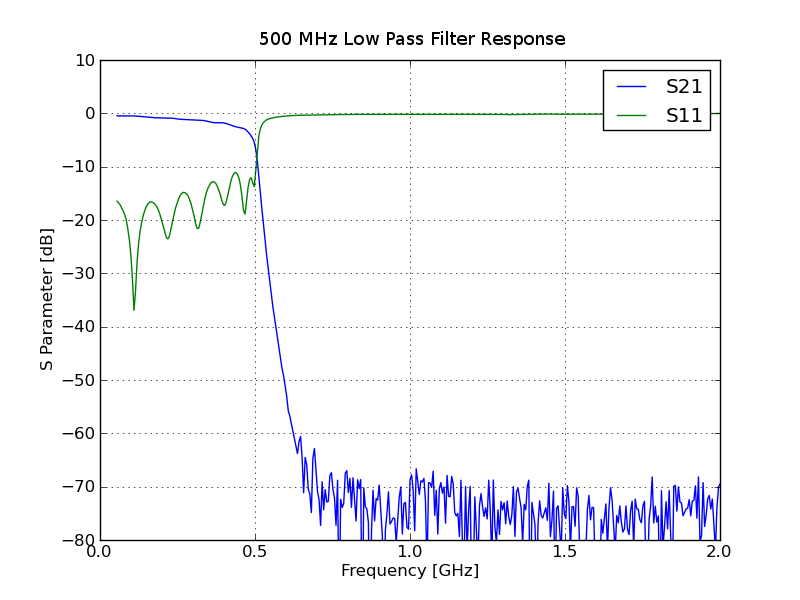
\includegraphics[width=0.5\textwidth]{./images/LowFrequencyFilters/LPF1.png}
%  \caption{The 0$\rightarrow$500MHz Low pass filter. }
%  \label{fig:LowFrequency0_500MHz}
% \end{figure}


 
\begin{figure}
 \centering
\subfloat[The 0$\rightarrow$500MHz Low pass filter.]{
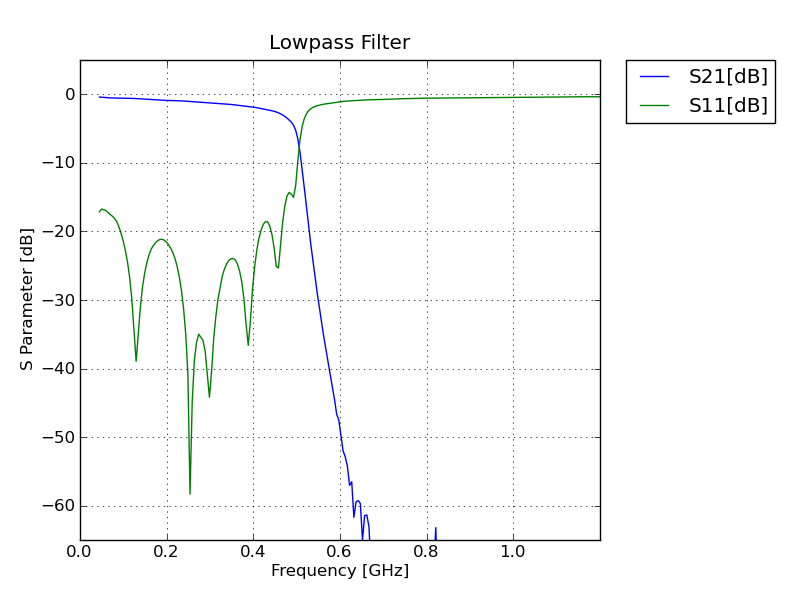
\includegraphics[width=0.5\textwidth]{./images/LowFrequencyFilters/LowpassFilter.png}
\label{fig:LowFrequency0_500MHz}
}\\
\subfloat[The 1000~MHz low pass filter ]{
 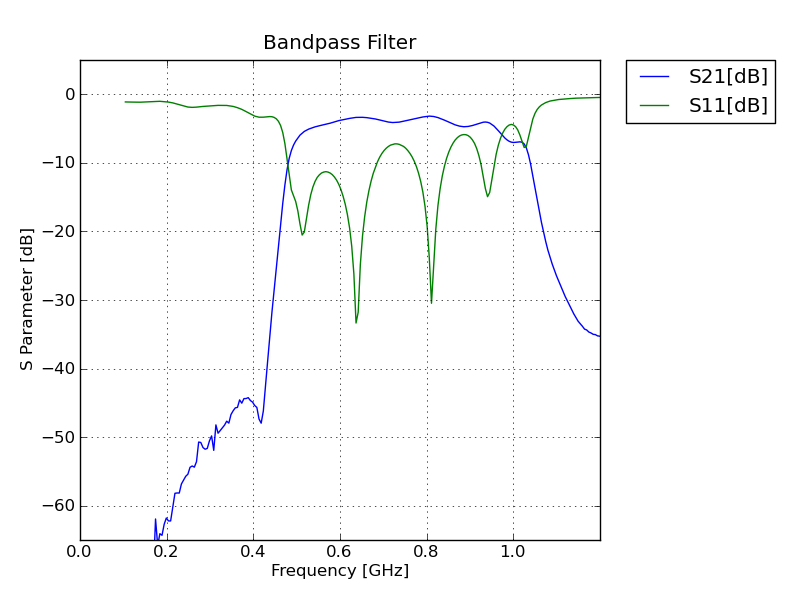
\includegraphics[width=0.5\textwidth]{./images/LowFrequencyFilters/BandpassFilter}
\label{fig:LowFrequency500_1000MHza}}
\label{fig:LowFrequencyFilters} 
\caption{The 500~MHz lowpass filter and the 500$\rightarrow$1000MHz bandpass filter. Since the bandpass filter operates at high frequenciess where lumped element design is difficult, we decided to make the band pass filter from a cascaded high pass filter (500MHz) and low pass filter (1000MHz). This allowed us to optimise the high end and low end independently. There is still a little work to do on the 1000~MHz filter (i.e the high end of the bandpass filter), but out understanding of these components' behavious at high frequency has improved significantly, and we believe this will be reflected in the next iteration}
\end{figure}


 \subsection{Component Choices}
At low frequencies filters are usually designed using surface mount or axial components. At low frequencies parasitic effects are negligible, however at higher frequencies the parasitic inductances and capacitances of the components need to be carefully considered during design. 

Many manufacturers release component libraries, which quantify these parasitics as well as other parameter changes with frequency. We chose to use Murata components, because of availability of suitable components in low quantities. 

Surface mount inductors can present significant challenges at high frequencies. Parasitic capacitance exists due to electric fields between small potential differences between the wire coils, and the wire itself presents a parasitic resistance. We tried the LQW18/LQW15 wire wound type inductors and the LQG18/LQG15 multilayer inductors \cite{murataInductors}. The manufacturing style of both is shown in \fign{fig:inductorStyles}. Both provide ranges from 1nH$\rightarrow$270nH and are designed for use at high frequencies.

\begin{figure}[ht]
 \centering
 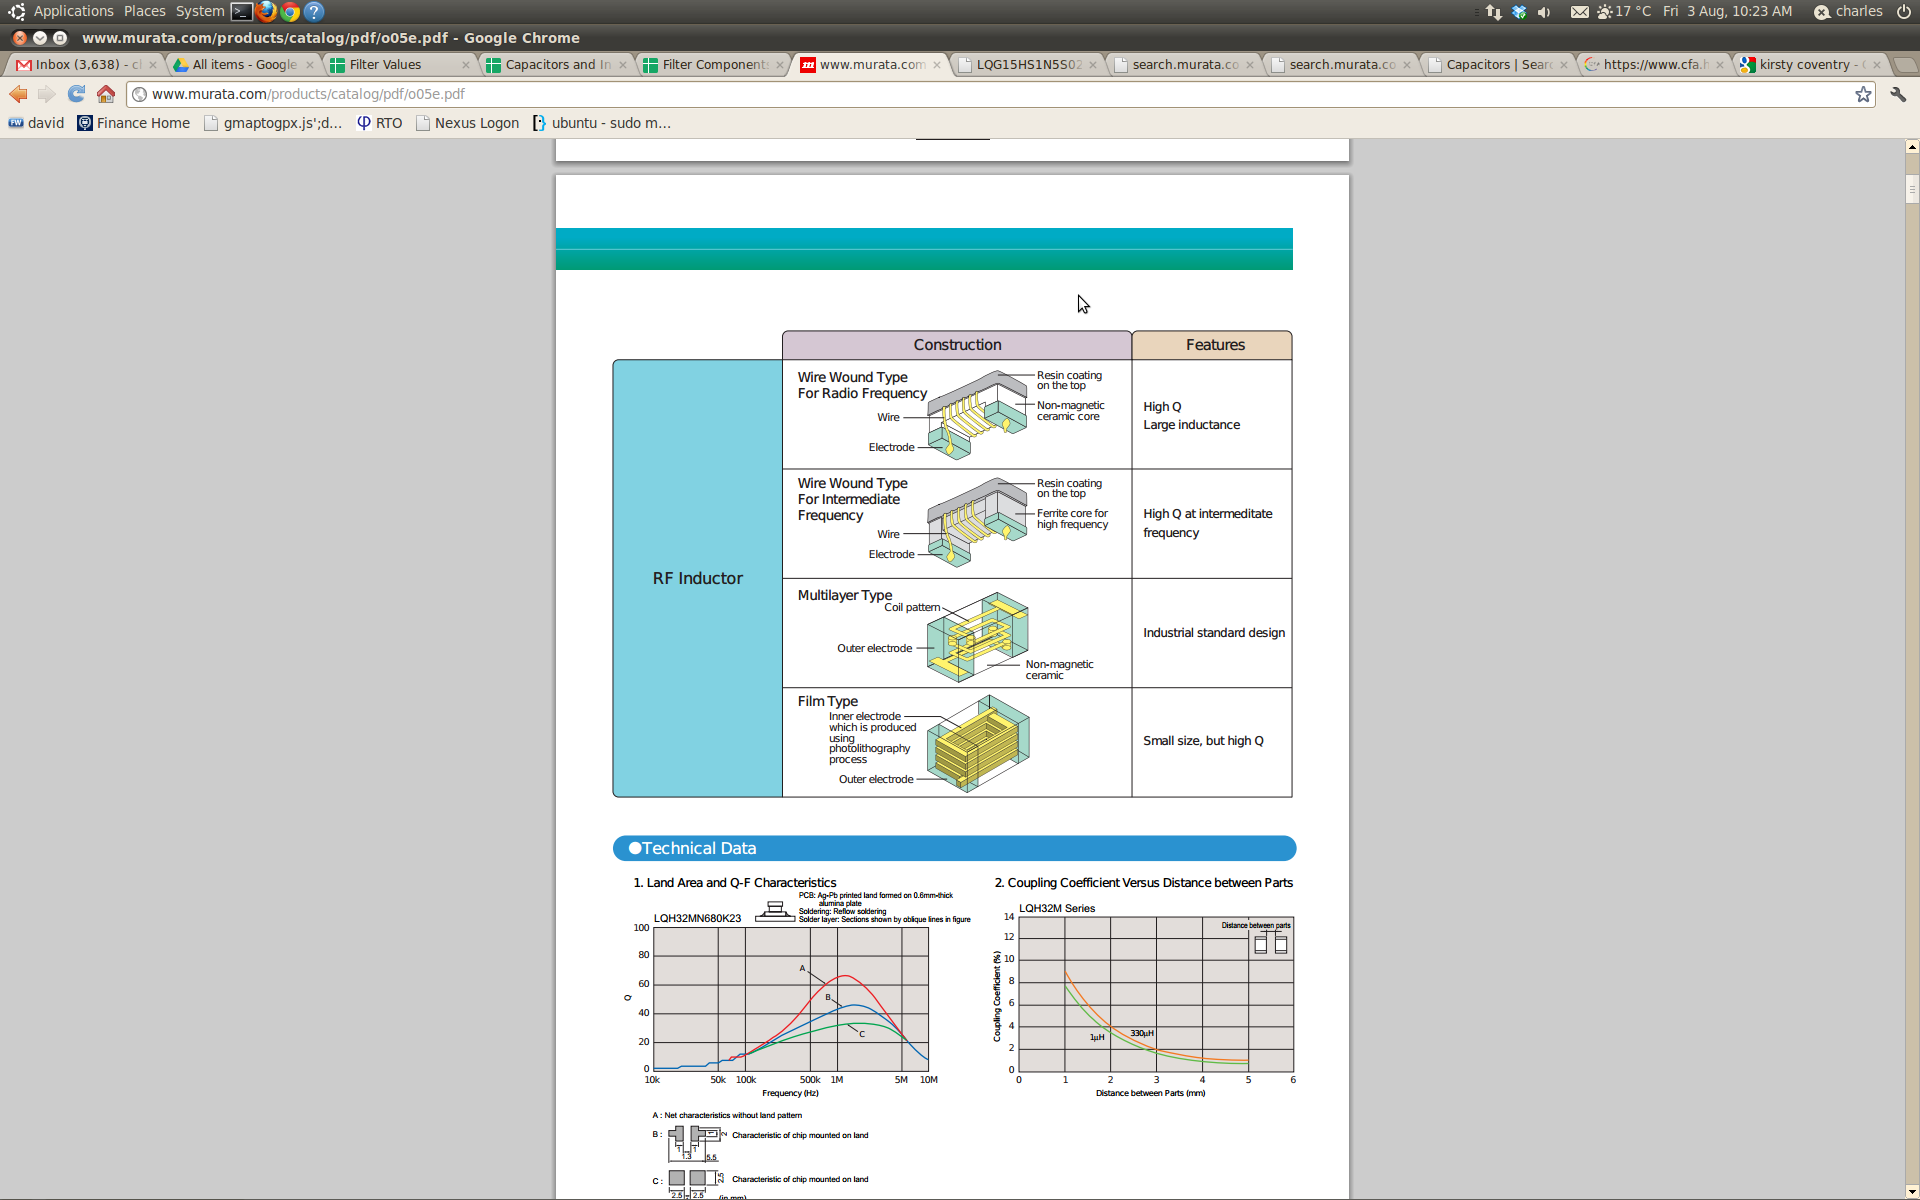
\includegraphics[width=\textwidth]{./images/LowFrequencyFilters/inductorStyles.png}
 % inductorStyles.png: 1920x1200 pixel, 72dpi, 67.73x42.33 cm, bb=0 0 1920 1200
 \caption{Different manufacturing styles of chip inductors \cite{murataInductors}}
 \label{fig:inductorStyles}
\end{figure}

For capacitors we chose the GJM15 Series ceramic capacitors also from Murata \cite{MurataCapacitors}. These are specifically designed for high frequency operations (up to 10~GHz), and are readily available across the full range of values from 0.1pF$\rightarrow$33pF. They feature low ESR (parasitic series resistance) (see \cite{MurataCapacitors} for values) 


  \subsection{Manufacture Techniques and Packaging}

Component choice is an important consideration, as is symmetry in the design. We have used coplanar waveguide to allow access to the ground plane on the top side of the board, and have laid out the components in a symmetrical fashion. As can be seen in \fign{fig:filterBoxing}, careful consideration also needs to be given to the way in which the filter boards are packaged. The packaging plays an important role in improving the out of band rejection characteristics.

\begin{figure}
 \centering
 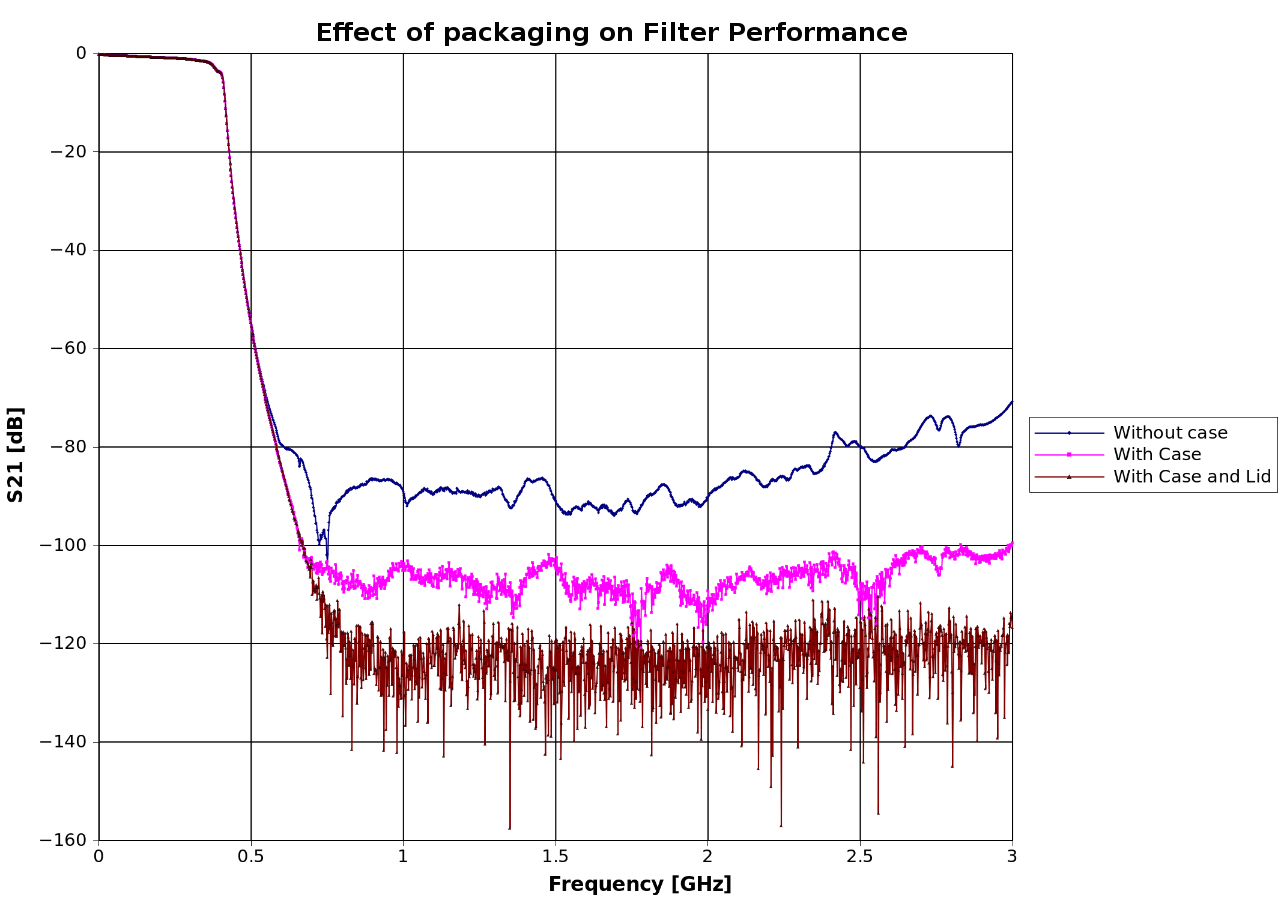
\includegraphics[width=\textwidth]{./images/LowFrequencyFilters/filterBoxing.png}
 % filterBoxing.png: 1319x930 pixel, 72dpi, 46.53x32.80 cm, bb=0 0 1319 930
 \caption{Comparison of different stages of the Filter construction process. These plots show the importance of properly enclosing the filter boards}
 \label{fig:filterBoxing}
\end{figure}

\begin{figure}
 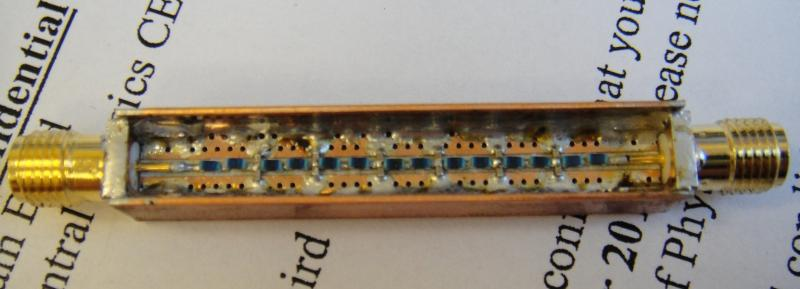
\includegraphics[width=\textwidth]{./images/LowFrequencyFilters/DSC03823a.jpg}
\caption{Final low frequency filter built into compact box. Notice the symmetry in the placement of components. The complete filter features a copper lid soldered into place completely sealing the unit. We have found that the boxing and lids are very important for optimal filter performance, as is apparent from \fign{fig:filterBoxing}. Also notice the solder joint between the PCB and the box wall. This reduces high frequency resonance artifacts, presumably caused by the (otherwise) exposed cavity}
\end{figure}

 

  \subsection{Performance}



\section{Double Sideband Mixers}

  \subsection{Design and Component Choice}

  \subsection{Performance}


\section{DC-6GHz Amplifiers}
Post down conversion gain is required to provide a suitable signal level at the ADC input. 


  \subsection{Performance}

  \subsection{Component Choice}

 \subsection{Wideband Biasing Chokes}

 \subsection{DC Blocking Capacitors}
DC blocking capacitors need to behave like series shorts in the frequency of interest. Capacitors can be modelled as a capacitor in series with a small, parasitic inductance and parasitic resistance \cite{Urs2011,broadbandCaps,Cain2010}. The impedance is then given by the equation in \eqn{eq:capacitorReactance}. This needs to be low (typically less than 1~ohm) across the frequency range of interest.

 \begin{eqnarray}
  X_{cap}=1/(2 \pi fC) + j 2 \pi fL + ESR
 \label{eq:capacitorReactance}
 \end{eqnarray}

Using \eqn{eq:capacitorReactance} large capacitor values are required for low frequency operation, while high frequency operation is limited by the parasitic inductance. 

As an example, at 5~MHz operation, a 100~nF capacitor has a reactance due to capacitance of 0.3~ohms, and a negligible 0.03~ohms contributed by typical parasitic inductances (0603 packaged MLCC capacitor has a typical parasitic inductance of 870~pH \cite{Cain2010}). However at 6~GHz the situation is reversed. The parasitic inductance now contributes 33~ohms, with the capacitance contribution of 0.0002~ohms being entirely negligible. The parasitic inductance is largely caused by the geometry of the package, with larger packaged featuring greater parasitic inductance. 

In order to achieve wideband performance from DC to 6~GHz, wideband DC blocking 0402 capacitors from American Technical Ceramics were used \cite{atc550L104}. The datasheet claims SRF of up to 40~GHz.

  
\section{Low Noise Amplifier Power Supply}

After the decision to move from the Jodrell Bank LNA's to Low Noise Factory LNA's, we required a means of powering the LNA's. Low Nois Facory do supply power supply units, however these do not allow remote monitoring. As such we built our own power supply units, in consultation with Low Noise Factory.

Extensive care was taken in components choice in order to minimise long term bias drifts. Many improvements were made in the original Low Noise Factory design, with particular care being taken to reduce any possible temperature drifts.

The basic schematic of the current source used in the power supply is included in 


\begin{figure}[ht]
 \centering
 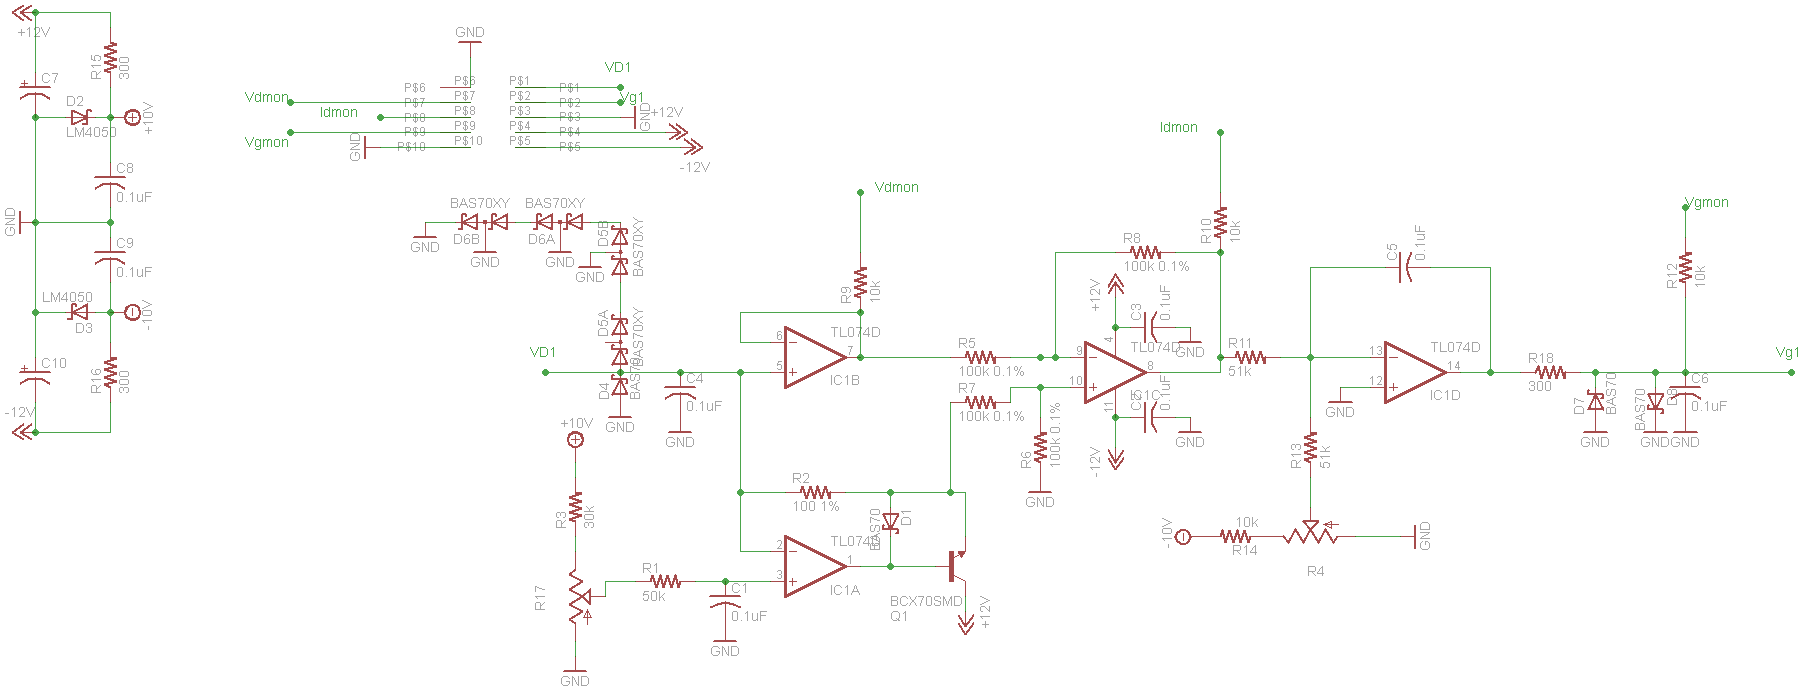
\includegraphics[width=\textwidth]{./images/LNAPSU/LNF-PS2_schematic.png}
 % LNF-PS2_schematic.png: 1807x692 pixel, 150dpi, 30.60x11.72 cm, bb=0 0 867 332
 \caption{The original amplifier power supply schematic. $\pm$10V reference was supplied by LM4050 Zener diode references (thermal stability 50ppm/\degc \cite{lm4050}), and TL074D opamps (Vo\approximately3000uV $\Delta$V$_{OS}$/$\Delta$C\approximately18uV/\degc \cite{tl074d}) were used for the gain and current stages . These were replaced by the more thermally stable REF195 voltage reference \cite{ref19x} and AD8624 opamps \cite{ad8624}. \fign{fig:lnaPSUNew} gives the schematic of the implementation. }
 \label{fig:LNFPowerSupply}
\end{figure}



\begin{figure}
 \centering
\subfloat[][New Power supply schematic]{
 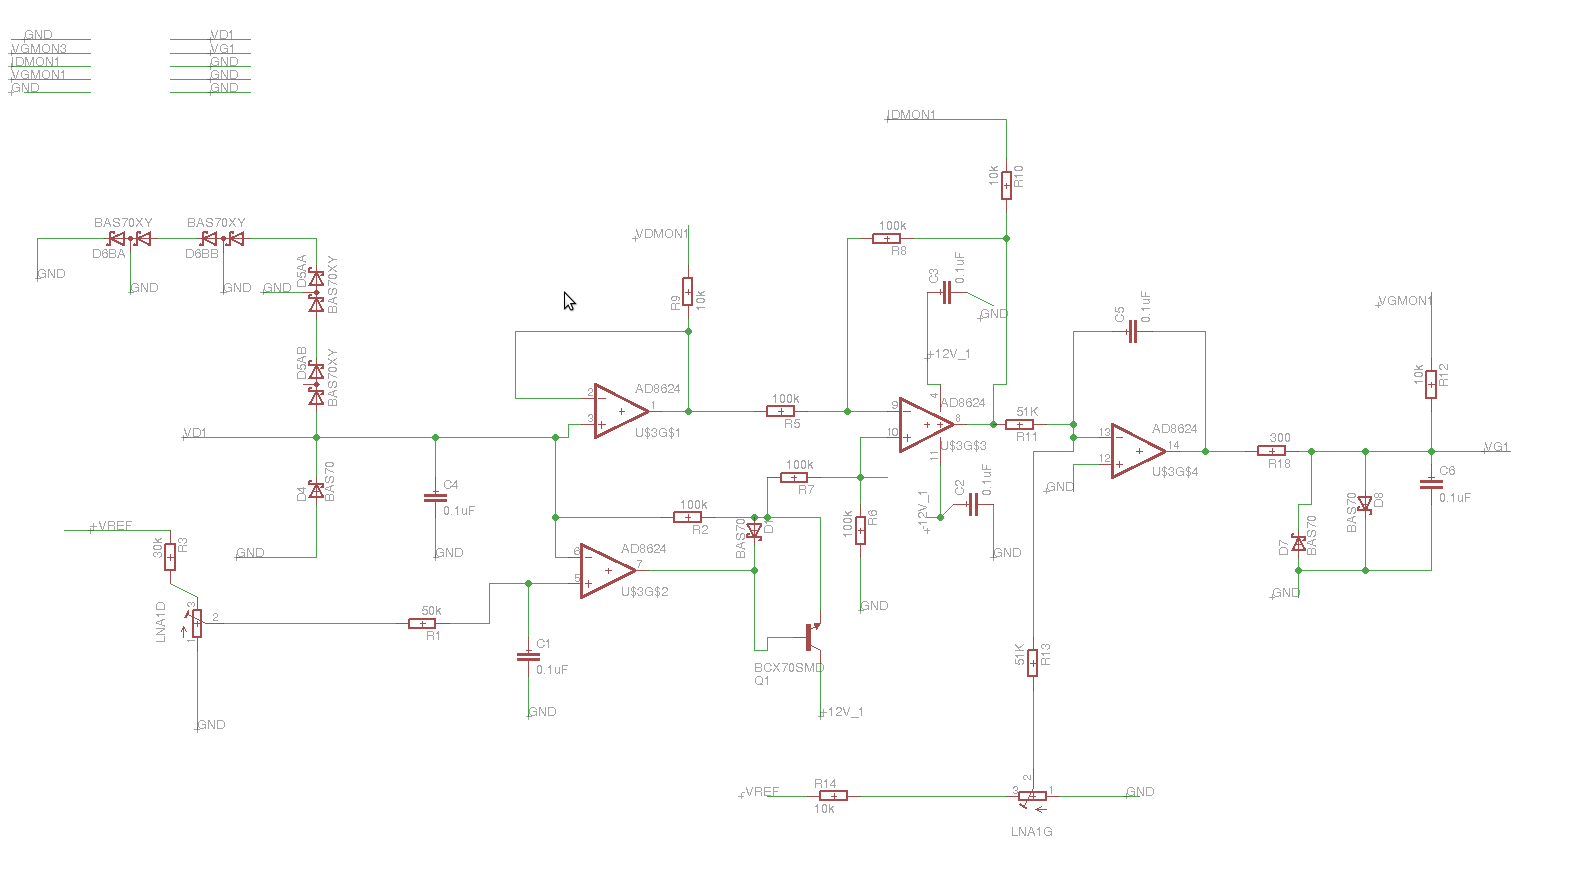
\includegraphics[width=\textwidth]{./images/LNAPSU/LNFNew.png}
\label{fig:NewPowerSupplyCircuit}
}\\
\subfloat[][New Reference voltage]{
 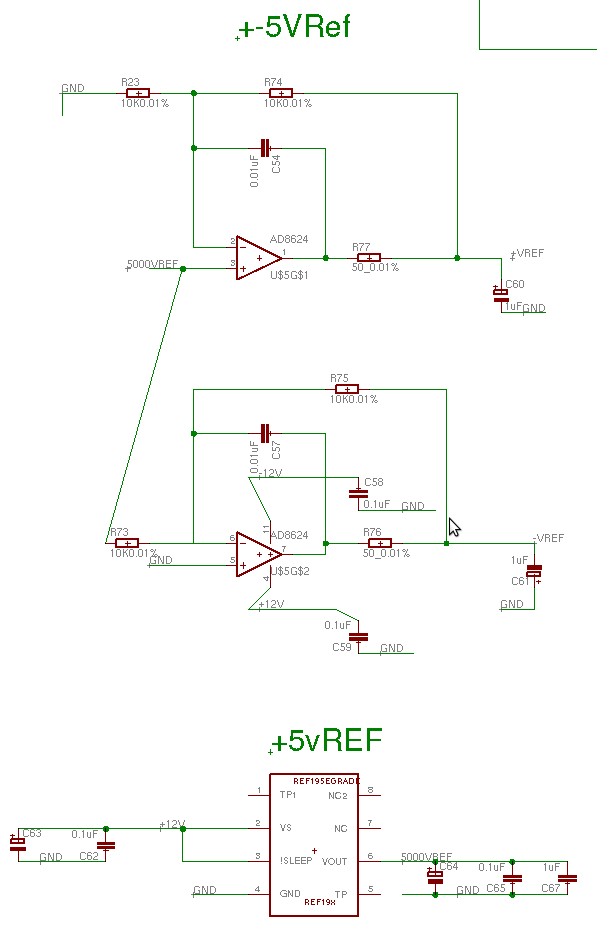
\includegraphics[height=0.4\textheight]{./images/LNAPSU/ReferenceSupply.png}
}\\

 % lowpass.png: 1357x340 pixel, 72dpi, 47.87x11.99 cm, bb=0 0 1357 340
 \caption{The updated-LNA Power Supply Board-The +5V reference voltage is provided by a REF195 E-Grade reference IC with a temperature coefficient of less than 5ppm/$^{\circ}$C \cite{ref19x}. The AD8624 opamps (Vo\approximately10uV $\Delta$V$_{OS}$/$\Delta$C\approximately1.2uV/\degc) \cite{ad8624} }
 \label{fig:lnaPSUNew}
\end{figure}







Replaced zener diode voltage reference generators, with REF19x units. Zener diodes 

